\chapter{Methodology}
\label{chap:Methodology}

This chapter describes the motivation and process behind performed experiments. It starts by describing our modified U-Net architecture and the challenges related to its training. The two following sections describe the preparation of the training data. The last section is a brief overview of object recognition metrics and it describes our motivation for using pixelwise F1 score as the evaluation metric.


\section{Architecture}
\label{sec:Architecture}

In the \emph{generative model} approach to semi-supervised learning, one usually starts with a model that can be trained in an unsupervised manner (either an autoencoder or a generative adversarial network; \cite{AutoencodersOverview}, \cite{GAN}) and then extends it to also perform the supervised task. For example, when starting with an autoencoder, one can use the encoder part as a dimensionality reduction mechanism and then build a supervised classification network that classifies the learned embeddings (\cite{KingmaSslVae}).

In our context of music recognition, we are highly motivated to build on top of the U-Net architecture (\cite{UNet}) (Figure \ref{fig:ArchitectureCombined}). It has first been used for biomedical image segmentation, however, its superiority for object detection in music recognition has been clearly demonstrated by \cite{PachaBaseline}.

The architecture can be viewed as a fully convolutional autoencoder with residual (skip) connections added between the encoder and decoder on every resolution level. The U-Net encoder is a typical fully-convolutional encoder that gradually reduces image dimensions while increasing the channel count. Such an architecture can learn abstract representations of symbols present in the input image. The decoder then tries to go from these abstract representations back to specific ones, while at the same time modifying the reconstruction to fit the learned segmentation task. The core idea behind this architecture is that the decoder can utilize skip connections during upsampling, thereby producing a pixel-perfect segmentation.

\begin{figure}[ht]
    \centering
    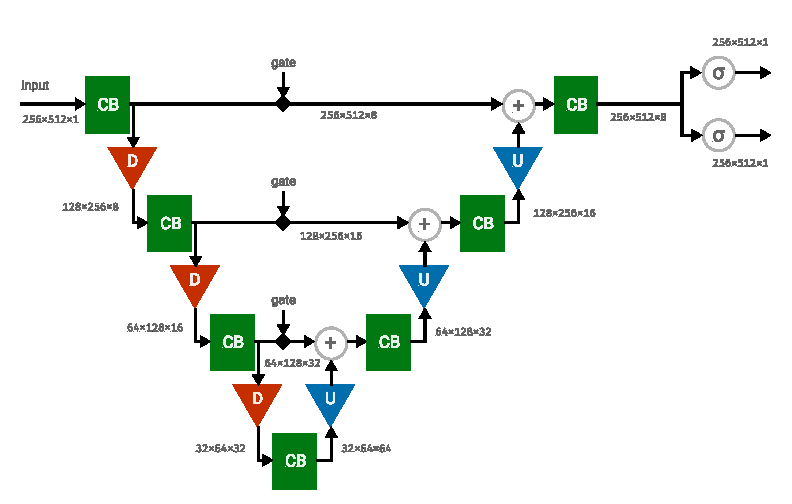
\includegraphics[width=145mm]{../img/architecture-complete.pdf}
    \caption{Block diagram, depicting the used architecture. It has 4 levels, with gated skip connections on each level. The network is forked after the second to last layer to provide separate segmentation and reconstruction outputs. A detailed explanation of each block is provided in Figure \ref{fig:ArchitecturePieces}.}
    \label{fig:ArchitectureCombined}
\end{figure}

We choose to share the entire U-Net model for both the supervised and unsupervised tasks. The two tasks are differentiated only at the very last layer. The original U-Net architecture ends with a 1x1 convolution layer with sigmoid activation. It can be viewed as a pixelwise softmax for two output classes (like in a typical classification architecture). We decided to fork the architecture here, having one sigmoid convolution for the supervised segmentation task and one for the unsupervised reconstruction task.

The supervised task can be trained in almost the same way as the original U-Net architecture:

\begin{itemize}
    \item A batch $(x, y)$ of input images and expected segmentation masks is taken from the dataset.
    \item Input images $x$ are fed through the model, producing a prediction for the segmentation mask $\hat{y}$ and for the reconstructed image $\hat{x}$.
    \item A loss function is used, computing the distance between $y$ and $\hat{y}$ and generating gradients for the network.
    \item Reconstruction output $\hat{x}$ is ignored and no gradients for the branch are computed.
    \item An optimizer uses computed gradients to update model parameters.
\end{itemize}

The unsupervised task can be trained in the same way, using the other output branch of the model. The model would receive an image on the input and would be trained to produce an identical image on the reconstruction output. This setup requires no labels, only the music images.

The unsupervised training, as described so far, would work for a typical autoencoder, but since the U-Net architecture contains skip connections, the model could learn an identity function without using any of the abstraction-learning layers. The goal of unsupervised learning is learning these abstract features, so this straightforward training scheme is infeasible in our context.

We propose two ways of overcoming this challenge:

\begin{itemize}
    \item gated skip connections
    \item denoising
\end{itemize}

One option is to disable skip connections during reconstruction training and keep them enabled during segmentation training. This should force the model to learn abstract features during reconstruction, while also being able to utilize skip connections during segmentation.

This gated scheme performs better than a plain autoencoder without any skip connections, but the experiment in Section \ref{sec:SkipConnections} suggests that having skip connections permanently enabled works better still. Despite this, we choose to use gated skip connections for reasons explained in that section. We combine this gating with the second technique of adding noise.

The denoising option refers to the process of adding noise to the input image when training the reconstruction task. The model learns to not only reconstruct the input image but also to remove the added noise. We took inspiration from denoising autoencoders (\cite{StackedDenoisingAutoencoders}). The difficult part is designing the noise function such that it would cause the model to learn abstract representations (see Section \ref{sec:NoiseGeneration}).

We consider the described scheme for unsupervised U-Net training to be the main contribution of this thesis. The proposed experiments try to assess the viability of the scheme in the context of semi-supervised learning.

Both the segmentation and reconstruction tasks are trained jointly on composite batches and a single composite loss function. A single optimizer step is used to update model parameters for both tasks simultaneously. The specifics of combining supervised and unsupervised training are described later in Section \ref{sec:Training}.

The last sigmoid layers output images with only one channel. For the reconstruction output, this data is interpreted as a grayscale image. For the segmentation output, it represents the probability the model assigns to each pixel of being in the target class. This means that the model can learn to segment only one symbol class.

\cite{HajicEtAl} have explored the option of having multiple segmentation output channels. The hypothesis is that having the model learn multiple classes would improve its accuracy since some internal representations can be shared. An added advantage is the reduced inference time as multiple segmentation masks can be inferred in a single pass. Such a training however introduces problems related to unbalanced class distribution in the training data. Even if these can be overcome, their results suggest minimal accuracy benefits and risk of decreasing accuracy in some cases.

Despite the fact that our experiments' source code lets us easily train multiple classes, we choose not to explore this path as we are interested in the semi-supervised effects only.

\begin{figure}[p]
    \centering
    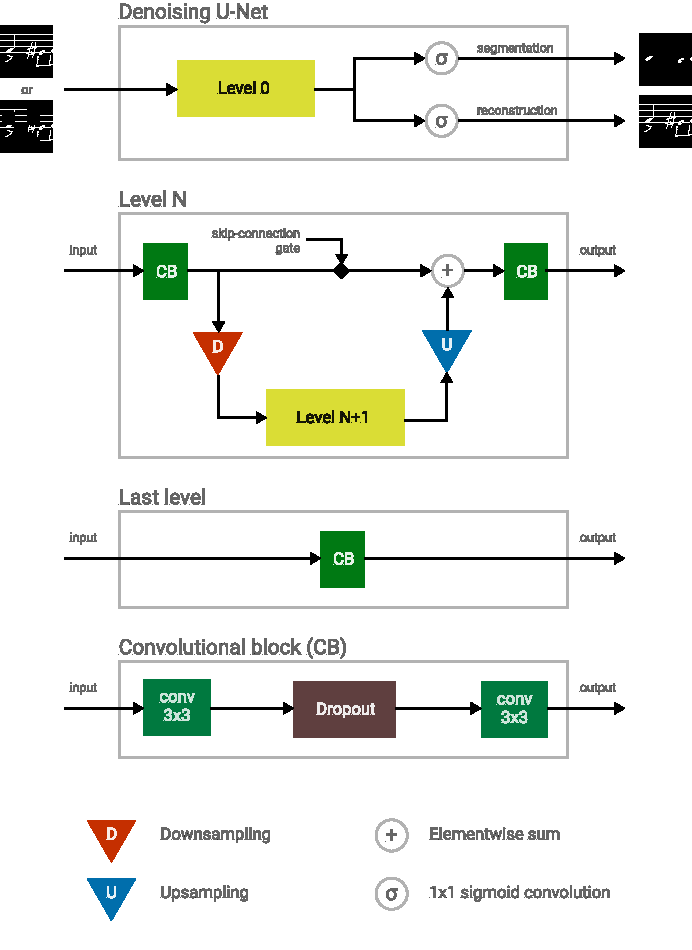
\includegraphics[width=145mm]{../img/architecture-pieces.pdf}
    \caption{A recursive block schema of the used architecture. When training and inferring segmentation, the input images are cropped directly from the given dataset. When training reconstruction, the input images are overlayed with large, tiled noise that zeroes out some pixels.}
    \label{fig:ArchitecturePieces}
\end{figure}

Figure \ref{fig:ArchitecturePieces} contains a recursive block diagram of our extended U-Net architecture. The model takes a single image as the input and produces both the segmentation mask and the reconstructed image. When training segmentation, the reconstructed image is ignored and when training reconstruction, the input image is covered in noise, and the output segmentation is ignored.

Each level of the network begins and ends with a convolutional block (CB). It consists of two identical 3x3 convolutional layers with an optional dropout layer in between them. Both convolutional blocks on the same level output the same number of feature channels. The number of feature channels is dictated by a hyperparameter we call \emph{inner features}. If the network has 4 inner features, the zeroth level convolutions output 4 feature channels. Each successive level then has twice as many feature channels as the one above it (e.g.\@ 4, 8, 16, 32). Figure \ref{fig:ArchitectureCombined} contains image dimensions and channel counts for each edge in the network. The image dimensions are taken for an input image tile of size 512x256.

The downsampling block is implemented as a 2D max-pooling layer (\cite{DeepLearningBook}). The number of feature channels is preserved. If we track the feature count through the encoder, we always first double the number of channels in the convolutional block and then reduce the spatial dimensionality in half in the downsampling block. This way the model can learn to extract higher-level features before the spatial resolution is lowered. Since the image is two-dimensional, halving the resolution shrinks the number of pixels to one quarter. Combined with the doubling of channel count, one encoder level effectively discards half of the image data. This acts as a bottleneck, forcing the network to learn relevant high-level representations.

The upsampling block has to perform two operations:

\begin{itemize}
    \item double the spatial dimensions
    \item halve the channel count
\end{itemize}

The resolution increase is performed by nearest neighbour interpolation (each pixel is copied to form a 2x2 region of the output image). The reduction in channel count is performed by a 1x1 convolutional layer, which can be trained to select or combine specific input channels. The upsampling output image may also be padded by zeros, if the desired output resolution is not even (we need to exactly match the resolution of the skip connection).

The gate on the skip connection is implemented as a multiplication by one or zero. This also causes any back-propagating gradients to be zeroed out, when the gate is closed. Implementation of this gating mechanism is inspired by LSTM and GRU cells used in recurrent neural networks (\cite{LSTM}, \cite{GRU}).

The output of the upsampling block and the skip connection is merged in an elementwise sum operation. The original U-Net paper uses concatenation (\cite{UNet}), however \cite{DorferEtAl} have shown that using a sum instead speeds up training, while having minimal impact on model accuracy.

In all layers (except for the two output sigmoid layers) the exponential linear unit (ELU) activation function is used. Reasons for this are described in Section \ref{sec:ActivationFunction}.


\section{Combining Datasets}

We need to slice and combine described datasets in various ways, depending on the performed experiment. There are two operations we want to perform:

\begin{itemize}
    \item Split an existing dataset into multiple slices (e.g.\@ validation, supervised and unsupervised slices).
    \item Combine two different datasets together.
\end{itemize}

The splitting is needed for an experiment, that gradually increases the amount of unlabeled data and measures the change in model accuracy. This means the splitting logic has to be stable with respect to the size of the unlabeled slice:

\begin{itemize}
    \item We do not want the content of other slices to change, when we change the size of the unlabeled slice.
    \item We want the unlabeled slice to only gain new data, not to be completely resampled.
\end{itemize}

This stability is achieved by giving consideration to the splitting logic (sampling the unlabeled data as the very last slice) and to the shuffling logic (the data is shuffled prior to splitting). All the randomness in the process is controlled by a parameter called \emph{dataset seed}, which is distinct from the plain \emph{seed} used for other initialization (model weights and noise generation). The introduction of the \emph{dataset seed} is essential for isolating our experiments from variability introduced by differential dataset sampling.

One additional consideration has to be made when sampling datasets CVC-MUSCIMA and MUSCIMA++. Because their content consists of music transcribed by 50 different writers, we want our splits to keep these writers separate. Another words, we do not want a single writer to be present in both the training set and the validation set. We enforce this constraint to better measure the ability of the trained model to generalize. The official test set of MUSCIMA++ built with this approach is called the \emph{writer-independent test set}, therefore we will call this property of our splitting logic \emph{writer-independence}.

\begin{figure}[ht]
    \centering
    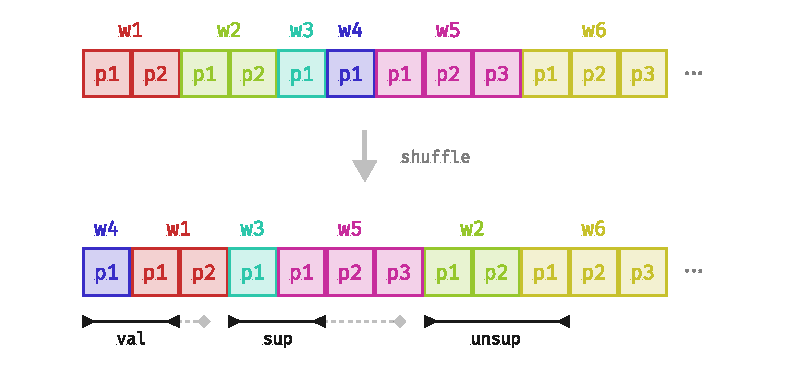
\includegraphics[width=140mm]{../img/dataset-splitting.pdf}
    \caption{Visualization of how a dataset is split in the writer-independent fashion, if we request 2 validation, 2 supervised and 3 unsupervised pages. (w) writer, (p) page}
    \label{fig:DatasetSplitting}
\end{figure}

When combining datasets, we run into the problem of image resolution. Since our proposed architecture learns visual features in a scale-dependent way, we need to bring all datasets to the same resolution. Datasets CVC-MUSCIMA and MUSCIMA++ have the same source images, so the problem is not present here, however, the dataset DeepScores is sampled at a lower resolution. In paper printing, a unit of DPI (dots per inch) is used. We cannot, however, use this unit, since it assumes the music from both datasets has the same size when printed on paper. A more general approach is to define a unit, that could be derived from the raster image itself, without any knowledge of the scanning/printing DPI. The open format MusicXML\footnote{\url{https://www.musicxml.com/}} uses a spatial unit defined as \emph{one tenth of interline space} (the distance between two adjacent stafflines). We took inspiration from this and defined a unit we call DPSS (dots per staff space). DPSS of a raster music document is the number of pixels between two neighboring stafflines. We measured the DPSS of CVC-MUSCIMA to be \verb`28.75 px` and of DeepScores to be \verb`16.0 px`.

\begin{figure}[ht]
    \centering
    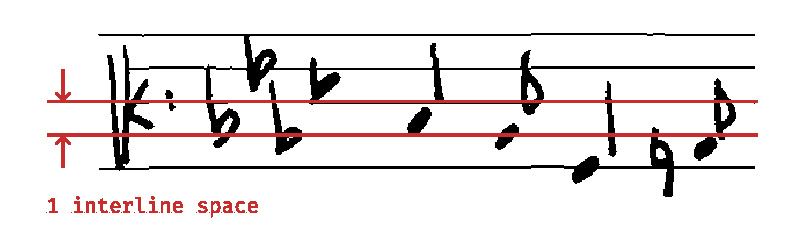
\includegraphics[width=140mm]{../img/dpss-definition.pdf}
    \caption{The spatial unit \emph{interline space}, size of which in pixels we call DPSS (dots per staff space).}
    \label{fig:DpssDefinition}
\end{figure}

When matching the resolution of both datasets, we need to perform image resizing and we need to choose the target size and the interpolation method. We ended up upscaling the DeepScores dataset to match the resolution of the CVC-MUSCIMA dataset with the bilinear interpolation method.

In the beginning, we tried downscaling CVC-MUSCIMA with the area interpolation method. We chose the area method because it does not produce aliasing artifacts (it works by averaging pixel values over an area). It, however, introduced problems with thin lines (such as stafflines and stems) that faded below 50\% intensity on most pixels. That caused the pixelwise F1 score we use to evaluate the experiments to become very noisy and difficult to interpret.


\section{Noise Generation}
\label{sec:NoiseGeneration}

Typical denoising autoencoders are used either for removing noise from existing images (say, an overlayed text, sensor noise, or aliasing artifacts) or for learning abstract features (\cite{StackedDenoisingAutoencoders}). If noise is sufficiently fine, so as to not obstruct the high-level structure of the image, the autoencoder can learn this high-level structure in an unsupervised way. This setup can be used for feature extraction, similar to how variational autoencoders are used (\cite{VariationalAutoencoder}).

\begin{figure}[ht]
    \centering
    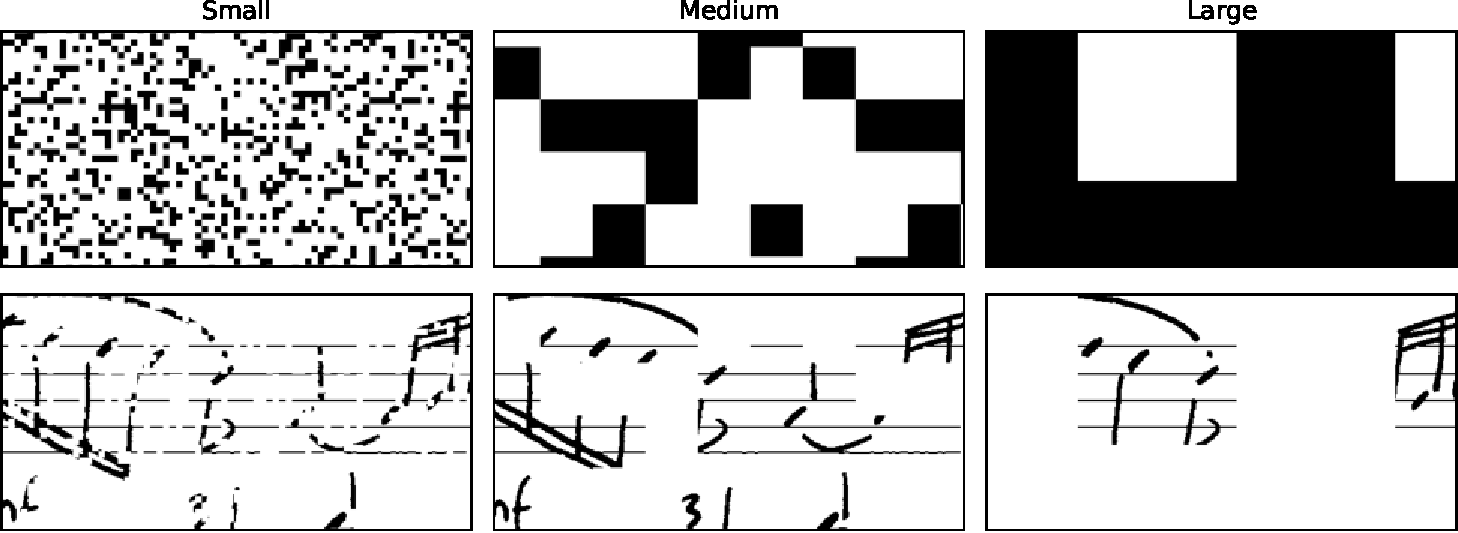
\includegraphics[width=145mm]{../../figures/06-noise/noise-comparison.pdf}
    \caption{Comparison of various noise sizes. Small noise is easy for the model to remove and large noise leaves too many possibilities of reconstruction.}
    \label{fig:NoiseComparison}
\end{figure}

Our goal is to leverage this training scheme to force our U-Net model to learn high-level representations. We chose to use noise in the form of dropping out parts of the input image -- setting the image pixels to zero. The parameter that specifies the percentage of the zeroed-out image area is called \emph{noise dropout}.

We could decide for each pixel independently, whether it should be dropped, but that would produce a very fine noise. We believe that such a noise would not force the model to learn large symbols, as they are unnecessary for removing the noise. Therefore we chose to increase the resolution of the noise to form a square grid, where one square covers approximately two staff spaces. At this size, dropped regions are large enough, so simple operations like dilation will not reconstruct them. These regions are also small enough that the number of plausible reconstructions within the dropped space is reasonably limited. An extreme situation would be dropping the entire input image, but there the space of possible reconstructions would be so large, that it would be impossible for the model to guess the correct one (even among the space of plausible reconstructions).

We got the idea of dropping image squares after reading the article by \cite{Cuneiforms}. The authors of the article present a method for reconstructing parts of an input image using a generative adversarial network. Their goal is to create synthetic training data for the task of cuneiform sign recognition.


\section{Evaluation Metrics}
\label{sec:EvaluationMetrics}

Semantic segmentation is closely related to object detection and recognition. It is often performed as the first step from which object bounding boxes are computed. The segmentation output is first binarized by applying a threshold. Adjacent positive pixels are merged to form connected components, where each can then be enclosed in a bounding box. The described process is very basic and there are ways to improve it. A slightly more advanced process in the context of notehead recognition is used in the article by \cite{DorferEtAl}.

There are many metrics that evaluate the correctness of predicted bounding boxes, comparing them to ground-truth bounding boxes. A metric called intersection over union (IOU) can be used to calculate the overlap of two bounding boxes. Setting a threshold on IOU and computing it between all pairs of predicted and ground-truth bounding boxes lets us compute the binary classification confusion matrix. From this matrix, additional metrics could be computed, such as precision, recall, and F1 score. By introducing a confidence level for each bounding box, or considering the performance over multiple classes, we get a large number of metrics that can be used to assess various aspects of the recognition. An article by \cite{PadillaMetrics} provides an extensive comparison of such metrics.

Even though these object detection metrics tell more about the actual usefulness of the model (we care about detected objects, not pixels), we chose to evaluate our experiments directly at the pixel level. Adding these evaluation metrics adds unnecessary complexity to our experiments and it is not needed for our goal -- measuring the impact of unsupervised data.

We chose to use the pixelwise F1 score at 0.5 thresholding. The F1 score is computed as the harmonic mean of precision and recall, so that it is high when both precision and recall are high. It is computed from the confusion matrix via the following formula:

$$
    F1 = \frac{2 \cdot TP}{2 \cdot TP + FP + FN}
$$

The confusion matrix values are computed over all pixels of the entire (validation) dataset.

It is important to note, that the two articles regarding music symbol detection (\cite{HajicEtAl}, \cite{DorferEtAl}) use object detection F1 score, which is not directly comparable to our pixelwise F1 score.
